%\documentclass[zihao=-4]{ctexbook} % 字号
\documentclass[UTF8, zihao=-4]{ctexart} % 字号
%强制字体设置 (use with xelatex)
%\setCJKmainfont{NSimSun}
%\setCJKmainfont{WenQuanYi Micro Hei}
%\setCJKmainfont{WenQuanYi Zen Hei}
%\setCJKmainfont{KaiTi_GB2312}

%if use with engine pdflatex: set the following
%\documentclass[UTF8, zihao=-4, zhmap=zhmCJK, fontset=none]{ctexart} % 字号
%\usepackage{zhmCJK}
%\setCJKmainfont{simsun.ttc}
%\setCJKsansfont{simkai.ttf}
%\setCJKmonofont{simfang.ttf}

\usepackage[colorlinks=false, backref=true]{hyperref} % PDF 目录
\usepackage{graphicx} % 包含图形文件
\usepackage{xcolor} % 颜色
\usepackage{geometry} % 版面边距
\usepackage{fancyhdr} % 定制页眉页脚

% 数学符号
\usepackage{amssymb}
\usepackage{amsmath}
\usepackage{mathrsfs}

\usepackage{multirow} % 多行表格
\usepackage{multicol} % 多列表格
\usepackage{animate} % PDF 动画
\usepackage{tabu} % 高级表格
\usepackage{listings} % 插入代码

\usepackage{extarrows} % 高级箭头
\usepackage[all]{xy} % 交换图表

% 参考文献库
\usepackage[backend=biber, style = caspervector, utf8]{biblatex}
% sorting: none 引用顺序 ecnty 英文在先 centy 中文在先
% 引用 \cite(supercite, parencite) [prenote][postnote]{key}
% prenote: 标号前置文字; postnote: 标号后置文字; key: 引用标签
% cite 无格式化标号 parencite [标号] supercite 上标标号
% \fullcite 打印完整参考文献条目
% 使用 biber -l zh__pinyin (zh__stroke) texfile 编译参考文献
% 打印文献列表: 
%     \printbibliography[title = {参考文献}, heading = bibnumbered]
%      title: 文献列表标题; 
%      heading: 
%           bibnumbered : 文献列表参与章节编号, 并被列入目录;  
%           bibintoc : 文献列表被列入目录中, 但不参与章节编号.

% 指定页面边距
\geometry{%
  a4paper,%
  top=2.5cm,%
  bottom=2.5cm,%
  left=3.2cm,%
  right=3.2cm%
}

% 指定章节标题
\ctexset {
      part = {
            name = {(,)}, % number 前的名字, number 后的名字
            % number 的样式 \chinese{part|section} 表示中文编号, \arabic 为数字
            % \Roman{...} 罗马数字, \roman{...} 小写罗马数字, \alph \Alph 小写, 大写字母
            number = {\chinese{part}}, 
            format = {\large\bfseries\color{blue}} % 文字样式: 大小+颜色
            % aftername = {\hspace{0.3cm}}
            % aftername 为章节编号与标题文本之间的内容
      },
      section = {
            format = {\large\rm\color{blue}}
      }
}

% 预定义常用数学符号
\newcommand{\real}{\mathbb{R}} % 实数
\newcommand{\comp}{\mathbb{C}} % 复数
\newcommand{\inte}{\mathbb{Z}} % 整数
\newcommand{\nat}{\mathbb{N}} % 自然数
\newcommand{\prob}{\mathbb{P}}
\newcommand{\expe}{\mathbb{E}}
\newcommand{\eps}{\varepsilon}
\newcommand{\four}{\mathscr{F}} %Fourier 变换
\newcommand{\co}{\mathcal{O}}
\newcommand{\id}{\text{Id}}
\newcommand{\im}{\text{Im}}
\newcommand{\End}{\text{End}}
\newcommand{\proof}{{\itshape 证明.}}
\newcommand{\lcode}{\lstinline} % 段内插入代码

% 小写罗马数字
\newcommand{\rmnum}[1]{\romannumeral #1}

% 定义新函数符号
\DeclareMathOperator*{\argmax}{\arg\,\max}

%mathbb 双透明体 (用于固定空间)
%mathbf 粗体
%mathcal 圆体 (用于算子)
%mathfrak 正体 (用于范畴)
%mathscr 花体 (用于集合系)

%\newtheorem{label}[共享编号来源(环境, 不是计数器)]{标题文本}[父计数器]
\newtheorem{theo}{定理}
\newtheorem{prop}{命题}
\newtheorem{problem}{算例}
\newtheorem{corollary}{推论}
\newtheorem{algorithm}{算法}

% 增加文献库
%\addbibresource{teng.bib}
%\addbibresource{tda.bib}

% 设置每个 part 重置 section 编号
%\makeatletter
%\@addtoreset{section}{part}
%\makeatother
%计数器命名: part, chapter(book), section, subsection, subsubsection, page,
%所有 newtheorem 定义的环境, equation, figure, table, footnote, 
%enum~(i, ii, iii, iv) 序列表环境中的编号.
%\setcounter{计数器}{值} 设置计数器的值.

% 设置页眉页脚

%\pagestyle{empty} %无页眉页脚
\pagestyle{plain} %首页页眉页脚
%\pagestyle{fancy} %定制页眉页脚

%\fancyhf{} %clear all head and foot
%\fancyhf[HF EO LCR,... (位置)]{内容} 数值页眉页脚
%H: Header F: Footer E: Even O: Odd L: left C: center R: right
%\renewcommand{\headrulewidth}{0.5pt} % width of head line
%\renewcommand{\footrulewidth}{0pt} % clear foot line
%\thetitle 标题 \thepage 页码 \thechapter \thesection 章节标题

% 修改名字为 plain 的页面样式 {} 内包含上一段中的命令
% 标题, 目录和章标题页面默认均为 plain 样式, 因此改变这些页面的样式只能使用本命令.
%\fancypagestyle{plain}{
%}

%\thispagestyle{plain} 改变当前页面的样式为 plain

\fancypagestyle{plain}{
      \renewcommand{\headrulewidth}{0pt} % width of head line
      \renewcommand{\footrulewidth}{0pt} % clear foot line
      \fancyhf[H]{}
      \fancyhf[FC]{\thepage}
}

\pagestyle{plain}

%重定义图表的引词
%\renewcommand\figurename{\rm 图}
%\renewcommand\tablename{\rm 表}

% 配置代码插入的风格
\lstset {
    language            =   go,                  % 代码语言
    basicstyle          =   \ttfamily,          % 基本代码风格
    keywordstyle        =   \color{blue}, % 关键字风格
    commentstyle        =   \ttfamily,  % 注释的风格,斜体
    stringstyle         =   \bfseries\ttfamily,  % 字符串风格
    flexiblecolumns,                % 别问为什么,加上这个
    %numbers             =   left,   % 行号的位置在左边
    %showspaces          =   false,  % 是否显示空格,显示了有点乱,所以不现实了
    %numberstyle         =   \zihao{-5}\ttfamily,    % 行号的样式,小五号,tt等宽字体
    showstringspaces    =   false,  % 是否显示 string 内部的空格
    captionpos          =   t,      % 这段代码的名字所呈现的位置,t指的是top上面
    frame               =   none,   % 显示边框, none: 不显示.
    breaklines          =   true,   % 自动换行
    columns             =   fixed,   
    basewidth           =   0.5em   % 字宽
}


\title{ftbt 战旗游戏引擎说明}
\date{最后更新日期: \today}
\author{滕飞}

\begin{document}
\maketitle

\section{引言}
\subsection{游戏基本流程}
\label{s_intro}
ftbt 是一款用 go 语言开发的回合制战棋游戏引擎, 是 20 世纪 90 年代颇为流行的游戏模式, 例如天使帝国, 三国英杰传等均属于该类型游戏. 
双方控制人物(棋子)在地图(棋盘)上移动并使用技术对对方人物造成伤害. 如果某人物的生命值 (HP) 被减少至零, 则从战斗地图中
退场 (移出棋盘). 首先将对方全部人物消灭的一方取得胜利. 双方轮流按回合进行游戏. 各方每回合的操作流程如下: 
\begin{enumerate}
      \item 置所有本方在场人物为未行动状态.
      \item \label{step_sel}选择一个尚未行动的人物进行操控.
      \item 计算该人物的允许移动范围.
      \item \label{step_move}选择该人物的移动目的地.
      \item 将该人物移动到目的地位置.
      \item \label{step_tech}选择该人物要使用的技能.
      \item \label{step_obj}选择该技能所针对的对象.
      \item 结算使用该技能的结果. 包括
            \begin{itemize}
                  \item 调整受影响人物的 HP
                  \item 判断并处置受影响人物是否离场
                  \item 判断游戏是否结束
            \end{itemize}
      \item 人物行动完成, 置已行动状态. 判断是否还有未行动本方人员, 有则转到第 \ref{step_sel} 步. 否则本操作方在本回合的行动结束.
\end{enumerate}
游戏共定义两个操作方, 分别编号 $0, 1$. 两操作方轮流执行一次记为一个回合.

\subsection{可执行程序}
\label{s_exec}
目前软件包内包括两个可执行程序: ftbt\_nc, ftbt\_nc\_ai. 
它们都使用了基于 NCurses 实现的 UI 前端. 其中 ftbt\_nc\_ai 为单人游戏, 即由人工操作一方, 由 AI 操作一方.
ftbt\_nc 为双人游戏, 即两方均由人工操作. 注意 AI 固定使用操作方 $1$.
其运行方法为
\begin{lstlisting}[language=bash]
ftbt_nc/ftbt_nc 规则文件 关卡文件 [关卡介绍文件]
ftbt_nc_ai/ftbt_nc_ai 规则文件 关卡文件 [关卡介绍文件]
\end{lstlisting}
其中, 规则文件和关卡文件的详细描述可参见第 \ref{s_conf} 节. 前端的操作说明可参见第 \ref{s_nc} 节.
关卡介绍文件包含关卡介绍的文本内容, 允许不提供.

\subsection{引擎使用}
游戏引擎的设计模式允许对同样的游戏规则设计不同的用户界面(UI). UI 通过 go 语言的 \lcode{interface} 结构来定义,
包括用于通知消息的 UI 接口 \lcode{UINote} 和用于获取用户操作的 UI 接口 \lcode{UISelect}.
接口的详细定义可参见第 \ref{s_ui} 节.
具体可按如下步骤使用.
\begin{enumerate}
      \item 用户需按 \lcode{UINote} 接口构造一个 \lcode{ui_note} 结构
      \item 用户需按 \lcode{UISelect} 接口构造两个结构, 可记为 \lcode{ui_select[2]}. 分别用于获取两个操作方的用户操作.
      \item 用户需调用函数
            \begin{lstlisting}
func Init (ui_note UINote, ui_select [2]UISelect, ftech, fmap io.Reader, fintro_name string) bool 
            \end{lstlisting}
            完成初始化引擎. 其中 ftech, fmap 分别为规则文件和关卡文件的读取接口. \lcode{fintro_name} 为关卡介绍文件的文件名.
            关卡介绍内容保存在 \lcode{intro string} 变量中. 如果 \lcode{len(intro) == 0}, 则采用 "No introduction" 作为
            关卡介绍内容.
      \item 如果需要启用 AI, 用户还需要依次调用
            \begin{lstlisting}
func InitAI ()
func LoadAI (ftech, fmap io.Reader) bool
            \end{lstlisting}
            来完成 AI 系统的初始化和加载配置. 此后, 在 \lcode{ui_select} 的相应接口中, 每次回合开始需调用
            \begin{lstlisting}
func AICalAllDist () 
            \end{lstlisting}
            来计算 AI 决策使用的距离信息.
            而在每个具体人物行动时, 需调用
            \begin{lstlisting}
func AIMakeDecision (ip int, move_loc []int)
            \end{lstlisting}
            来获得 AI 决策结果. 其中 \lcode{move_loc} 为所有可能的移动目的地数组, 在 \lcode{ui_select} 接口中可获得.
            决策结果返回到
            \begin{lstlisting}
ai_people[ip].opt_move_loc
ai_people[ip].opt_tech_obj
            \end{lstlisting}
            分别表示第 \lcode{ip} 号人物的决策移动目的地和决策技术目标. 若 \lcode{ai_people[ip].opt_tech_obj} 为 $-1$,
            则表示该人物仅做移动, 不执行技术.
      \item 调用函数  
            \begin{lstlisting}
func Do () (st int)
            \end{lstlisting}
            来启动引擎, 游戏结束后该函数返回. 返回值包括
            \begin{lstlisting}
const (
	TST_WIN = 0
	TST_LOSS = 1
	TST_QUIT = 2
)
            \end{lstlisting}
            其中, \lcode{TST_WIN} 表示操作方 $0$ 获胜, \lcode{TST_LOSS} 表示操作方 $1$ 获胜. \lcode{TST_QUIT} 表示用户中途退出.
\end{enumerate}

\section{游戏详细规则}
\subsection{人物属性}
每个人物包括如下定义的属性.
\begin{lstlisting}
type People struct {
	name string
	opt int

	abi int
	def int

	hp int

	tech []int

	speed int

	loc int
	is_finish bool
}
var people []People
\end{lstlisting}
其中, \lcode{name} 为人物的姓名. \lcode{opt} 取值 $\{0, 1\}$, 用于表示人物所属于两个阵营中的哪一个.
对于有 AI 加入的情形, \lcode{opt = 0} 表示由人工操控的一方, \lcode{opt = 1} 表示由 AI 操作的一方.
\lcode{abi} 为攻击力数值,  \lcode{def} 为防御力数值, \lcode{hp} 为生命值, 
\lcode{tech} 表明所允许使用的技术集, 取值为总技术集中的索引编号. 
\lcode{speed} 为每次移动的总移动量, \lcode{loc} 为人物所在地图上的位置. 如果人物撤离战场, 则取 \lcode{loc = -1}.
设地图在 $x, y$ 两个方向的格子数分别为 $n_x, n_y$, 则可用两种方法表示地图上的一个位置. 
一种是使用二维坐标 $(x, y), x, y \in \inte_+$, 另一种是根据公式
\begin{equation}
      \label{e_loc}
      l := yn_x + x
\end{equation}
计算得到一个整数值 $l \in \inte_+$. 此处的 \lcode{loc} 取后者. 本文中提到所有的单一位置编号均按后者理解.

\lcode{people} 数组维护了所有人物属性的结构.

\subsection{地图与移动规则}
地图类似围棋棋盘, 由 $n_x \times n_y$ 个网格组成. 每个格子被赋予特定的地形, 每种地形被赋予特定的移动消耗值 (\lcode{weight}).
如此, 地图上每个格子都关联上了唯一的 \lcode{weight}. 具体的, 每个地图网格包含如下定义的属性.
\begin{lstlisting}
type Location struct {
	people int
	dx int
	weight int

	/* 用于指示路径和是否有效: -1: 起点, 有效, -2: 无效 
	* 移动时指示路径中的上一个点 */
	path_last_loc int 

	/* [操作方][攻防] */
	buf_value [2][2] int
	buf_dur [2][2] int
	fly_weight [2]int
	fly_weight_dur [2]int
	disable_long [2]bool
	disable_long_dur [2]int
}
var gmap []Location 
var dx_weight [] int
var dx_name []string

\end{lstlisting}
其中, \lcode{people} 指明占据该网格的人员编号, 无人则取 $-1$. \lcode{dx} 为该网格的地形编号, 
\lcode{weight} 为与网格关联的移动量消耗值. \lcode{gmap} 维护所有位置的结构, 其中位置的顺序按照 (\ref{e_loc}) 中 $l$ 从小到大排列. 
\lcode{dx_weight} 保存所有地形的移动量消耗值, \lcode{dx_name} 保存所有地形的名称.

当地图上划定了一个选择范围时, 可通过 \lcode{path_last_loc} 属性获得该范围. 
当 \lcode{path_last_loc} 为 $-2$ 时, 表示该位置不属于有效范围, 否则属于有效范围.  
当标记人物可移动的范围时, $-1$ 表示人物移动的起点, 一个非负值表示该位置在最短移动路径
上的上一步的位置. 当标记技术目标的选择范围时, 只使用 $-1$ 表示该位置有效.

\lcode{buf_value} 和 \lcode{buf_dur} 数组用于指示该网格的攻防辅助效果. 
注意对两个操作方有不同的辅助效果.
两个维度的含义分别为 \lcode{[操作方][攻防]}, 其中 $0$ 表示攻, $1$ 表示防.
\lcode{buf_value} 为实际的辅助攻防值, \lcode{buf_dur} 为效果的剩余持续时间.

\lcode{fly_weight} 和 \lcode{fly_weight_dur} 数组用于指示该网格的飞行辅助效果, 即修改网格的移动消耗量.
维度的含义为操作方. \lcode{fly_weight} 用于表明修改后实际的移动消耗量. \lcode{fly_weight_dur} 为效果的剩余持续时间.
与 \lcode{fly_weight} 和 \lcode{fly_weight_dur} 的含义类似, \lcode{disable_long} 和 \lcode{disable_long_dur} 
数组用于指示远程攻击无效的辅助效果. 其中, \lcode{disable_long} 为 \lcode{true} 表明辅助效果启动.

每个人物被赋予一定的移动速度 (\lcode{speed}), 即每回合开始移动前
的保存移动量. 人物允许从地图上一个格子移动到相邻四个格子中的其中之一, 每移动一格将消耗一定的移动量. 消耗量等于目的地格子的
\lcode{weight}. 根据每个人的 \lcode{speed} 和每个格子的 \lcode{weight} 就可通过 Dijkstra 算法计算出允许的移动范围和到达
每个允许目的地的最短路径及消耗移动量. 还包括如下特殊规则.
\begin{itemize}
      \item 所有已经被其他人占据的格子无法作为移动目的地.
      \item 被本方人物占据的格子可以位于移动路径中, 但被敌方人物占据的格子不得位于移动路径中
      \item 当如图\ref{f_go_by}所示从侧向经过敌方人物相邻的格子时, 所消耗的移动量为该格 \lcode{weight} 的一定倍数 
            (由常数 \lcode{NEIGHBOUR_WEIGHT_SCALE} 所指定).
\end{itemize}
\begin{figure}
      \begin{center}
            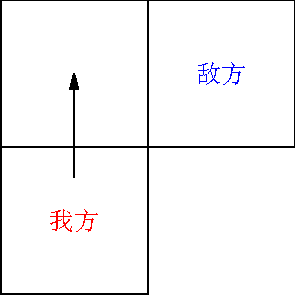
\includegraphics[scale=1]{go_by.pdf}
      \end{center}
      \caption{\label{f_go_by}侧向经过敌方人物邻接格子示意}
\end{figure}

\subsection{技能规则}
人物可使用的技能被分为 $5$ 类. 由如下常数定义.
\begin{lstlisting}
const (
	TC_PEOPLE = 0
	/* 时间, 范围均不可变 */
	TC_ABI_BUF = 1
	TC_DEF_BUF = 2
	/* 时间固定, 范围可变 */
	TC_FLY = 3
	/* 时间, 范围均可变 */
	TC_DISABLE_LONG = 4
)
\end{lstlisting}
\lcode{TC_PEOPLE} 类为直接对敌方人物的 HP 造成伤害的技能, 目标对象必须为敌方人物. 
该类技能又被分为近体技能和远程技能.
其余 $4$ 类技能的目标对象为地图上的一个位置. 他们的目的是对地图上的一部分区域提供有利于己方的辅助效果.
具体的, \lcode{TC_ABI_BUF} 用于辅助提升己方攻击力. \lcode{TC_DEF_BUF} 用于辅助提升己方防御力.
\lcode{TC_FLY} 用于减少己方人物移动经过相应位置所消耗的移动量.
\lcode{TC_DISABLE_LONG} 用于使己方人物在特定区域内免除敌方的远程技能伤害.

具体的, 每个技能包括如下属性定义.
\begin{lstlisting}
type Tech struct {
	name string
	class int
	/* 是否为远距离 */
	is_long bool
	/* 可选择的作用范围 */
	rel_range [][2]int
	/* aoe 范围, 可变时,表示最大值 */
	aoe_range int
	/* aoe 比例 (%)*/
	aoe_ratio int
	/* aoe 是否影响己方单位 */
	aoe_self bool
	/* 持续时间, 可变时, 表示最大值 */
	duration int
	/* 支持地形 */
	dx []bool

	/* 效果值:
	* 对于 TC_PEOPLE, 为基础伤害值, 
	* 对于 其他类型, 为使用者 abi 的百分比值
	*/
	value int

}

var gtech []Tech
\end{lstlisting}
其中, \lcode{name} 为技能名称, \lcode{class} 为技能类型, 
\lcode{is_long} 用于指示该技能是否为远程技能,
\lcode{rel_range} 用于指示第\ref{s_intro}节所述第\ref{step_obj}步可选择技能目标的范围.
这是一个数组, 每个元素表明一个相对于技能施放者的相对位置.
\lcode{aoe_range} 用于指示技能作用到目标后, 作用范围的延展范围, 即以作用目标为中心, 
技能可以影响作用目标周围距离作用目标不大于 \lcode{aoe_range} 的网格.
技能对于延展范围内的目标的作用效果相对于主目标会存在衰减.
\lcode{aoe_ratio} 为一个百分比 ($100$ 为上限), 用于表明技能对于延展范围内的目标的作用效果与对中心目标的作用效果的比值, 以衡量上述衰减. 
\lcode{aoe_self} 表明技能在延展范围内是否会影响到己方人物, 仅在类型为 \lcode{TC_PEOPLE} 时有意义.
\lcode{duration} 仅对除 \lcode{TC_PEOPLE} 类型外的技能有意义, 用于表明添加到地图区域的辅助效果的持续时间.
\lcode{dx} 用于对技术目标所在地的地形进行限制. 数组大小等于地形的个数, 取值 \lcode{true} 表明该技术在对地形有效, 否则为无效.
无论通过 \lcode{rel_range} 所确定的范围选择主要技术目标, 还是通过 \lcode{aoe_range} 自动选择延展范围内的作用目标, 均受该地形限制的影响.
\lcode{value} 为技术的效果值, 对于不同类型的技术含义不同, 以下会具体说明. \lcode{gtech} 维护了所有技能的结构.

下面具体说明每种类型技术的效果. 
\begin{description}
      \item [TC\_PEOPLE] 
            对主目标造成 $$ \text{施用者攻击} - \text{目标防御} + \text{技术效果值} $$ 的伤害.
            如果 \lcode{aoe_self} 为 \lcode{true}, 则考虑延展范围内的所有人物, 
            否则只考虑延展范围内的敌方人物, 将其作为延展目标.
            对延展目标造成的伤害为 $$ \text{主目标伤害} \times \text{aoe\_ratio} / 100. $$
            注意上述计算攻击和防御时还需要考虑施用者所在位置的攻击辅助加成和受害者所在位置的防御加成.
      \item [TC\_ABI\_BUF 和 TC\_DEF\_BUF]
            对主目标位置造成 $$ \text{施用者攻击} \times \text{技术效果值} / 100 $$ 的辅助加成.
            对所有延展范围内的位置造成 $$ \text{主目标位置辅助加成} \times \text{aoe\_ratio} / 100 $$ 的辅助加成.
            \lcode{TC_ABI_BUF} 对应攻击加成, \lcode{TC_DEF_BUF} 对应防御加成. 注意加成仅在己方回合内有效.
            加成持续的回合数为 \lcode{duration}.
      \item [TC\_FLY]
            设主目标技术值 $$ \text{abi} := \text{施用者攻击} \times \text{技术效果值} / 100, $$ 
            延展目标技术值 $$ \text{abi\_e} := \text{abi} \times \text{aoe\_ratio} / 100 $$
            则主目标位置的移动量消耗值将被修改为
            \begin{lstlisting}
weight = (MAX_FLY_WEIGHT - 1) * (MAX_ABI - abi) / MAX_ABI + 1
            \end{lstlisting}
            延展范围内的有效位置的移动量消耗值将被修改为
            \begin{lstlisting}
weight = (MAX_FLY_WEIGHT - 1) * (MAX_ABI - abi_e) / MAX_ABI + 1
            \end{lstlisting}
            其中, \lcode{MAX_FLY_WEIGHT} 和 \lcode{MAX_ABI} 为两个常数, 用户可在配置文件中指定, 参见第\ref{s_conf}节.
            目标移动量变化持续的回合数为 \lcode{duration}.
            本类技术的延展范围半径也与释放者有关, 具体按公式
            \begin{lstlisting}
aoe_dist := tech.aoe_range * p.abi * tech.value / (100 * MAX_ABI)
            \end{lstlisting}
            计算. 其中 \lcode{p.abi} 为释放者的攻击力. \lcode{tech.aoe_range} 和 \lcode{tech.value} 为技术相关属性.
      \item [TC\_DISABLE\_LONG] 
            目标位置及延展范围内的所有位置均被设置为屏蔽远程攻击. 
            延展范围的半径和效果持续时间均与释放者有关, 具体按公式
            \begin{lstlisting}
aoe_dist := tech.aoe_range * p.abi / MAX_ABI
dur := tech.duration * p.abi / MAX_ABI
            \end{lstlisting}
            来计算. 其中, \lcode{aoe_dist} 为延展范围半径, \lcode{dur} 为屏蔽效果持续时间, \lcode{tech.duration} 为技术相关属性.
\end{description}

\section{配置文件说明}
\label{s_conf}
游戏运行需要提供配置文件, 包括规则文件和关卡文件. 配置文件为纯文本文件, 采用 UTF-8 编码. 
内容为以空白字符 (空格, 换行, Tab) 分割的文本数据. 数据类型有整数, 字符串和逻辑值. 
其中逻辑值表述为 true 或 false.
\subsection{规则文件}
以下依次介绍规则文件中的各项数据值的含义和类型.
\begin{enumerate}
      \item 地形的个数 (整数)
      \item 依序对每一种地形, 依次为
            \begin{enumerate}
                  \item 地形名称 (字符串)
                  \item 地形消耗的移动量 (整数)
            \end{enumerate}
      \item \lcode{MAX_FLY_WEIGHT} (整数)
      \item \lcode{MAX_ABI} (整数)
      \item 总技能个数 (整数)
      \item 依序对每个技能指定属性
            \begin{enumerate}
                  \item 技能名称 (字符串)
                  \item 技能类型 (整数)
                  \item \lcode{is_long}
                  \item 主目标相对范围 (\lcode{rel_range}) 中包含的位置个数 (整数)
                  \item 对\lcode{rel_range}中的每个位置
                        \begin{enumerate}
                              \item 位置的 x 坐标 (整数)
                              \item 位置的 y 坐标 (整数)
                        \end{enumerate}
                  \item \lcode{aoe_range} (整数)
                  \item \lcode{aoe_ratio} (整数)
                  \item \lcode{aoe_self} (逻辑值)
                  \item \lcode{duration} (整数)
                  \item \lcode{dx} : 即技能是否能在每种地形上(作为主目标位置)施放. 对每种地形
                        \begin{enumerate}
                              \item 是否允许作为主目标及延展目标 (逻辑值)
                        \end{enumerate}
                  \item \lcode{value} (整数)
            \end{enumerate}
      \item 以下配置参数与 AI 相关, 包括
            \begin{lstlisting}
AI_MAX_MOVE_DIST int
AI_MAX_MOVE_SCORE int

AI_MAX_BUF_VALUE int
AI_MAX_BUF_SCORE int

AI_MAX_DEF_DIST int
AI_MAX_DEF_SCORE int

AI_MAX_TECH_DIST int
AI_MAX_TECH_SCORE int

AI_MAX_TECH_BUF_VMD int
AI_MAX_TECH_FLY_VMD int
AI_MAX_TECH_DL_DUR int
            \end{lstlisting}
            它们用于在 AI 做出决策时对人物可能的行为进行评分, 取分值最大的行为作为最终的执行策略. 具体的,
            \begin{itemize}
                  \item \lcode{AI_MAX_MOVE_DIST} 和 \lcode{AI_MAX_MOVE_SCORE} 用于决定移动目的地的位置评分, 
                        关卡文件中会为每个 AI 人物指定一个目标位置. 每次AI人物行动时, AI 会计算移动目的地距离目标位置
                        的移动量消耗 $d$, 如果 $d = 0$, 则评分为 \lcode{AI_MAX_MOVE_SCORE}.
                        如果 $d = \text{\lcode{AI_MAX_MOVE_DIST}}$, 则评分为 $0$. 评分与 $d$ 呈线性关系.
                  \item \lcode{AI_MAX_BUF_VALUE} 和 \lcode{AI_MAX_BUF_SCORE} 用于决定移动目的地的辅助攻防评分.
                        如果目的地的辅助攻击(防御)达到 \lcode{AI_MAX_BUF_VALUE}, 则获得评分 \lcode{AI_MAX_BUF_SCORE},
                        如果没有辅助攻击(防御), 则获得零评分. 所获得的评分与目的地的辅助攻防值呈线性关系.
                  \item \lcode{AI_MAX_DEF_DIST} 和 \lcode{AI_MAX_DEF_SCORE} 用于决定移动目的地的防御评分.
                        AI 会计算目的地与每个敌人的距离(按消耗移动量计算). 如果距离达到 \lcode{AI_MAX_DEF_DIST},
                        则记该敌人的评分为 $0$. 如果距离为零, 则记该敌人的评分为 \lcode{AI_MAX_DEF_SCORE}.
                        每个敌人的评分均与目的地距敌人的距离呈线性关系. 最终该目的地的防御评分为所有场上敌人的防御评分
                        的平均值.
                  \item 以下按照技术类型分别说明 AI 对使用技术的评分计算. 这需要在给定目标位置(人物)的前提下进行.
                        对于除 \lcode{TC_PEOPLE} 类以外的技术, 需要首先对每个延展范围内的位置计算如下距离差.
                        \begin{lstlisting}
inv_gd := AI_MAX_TECH_DIST - aip.goal_dist[loc]
                        \end{lstlisting}
                        其中 \lcode{aip.goal_dist[loc]} 表示待计算的技能影响位置与 AI 当前操作人物的目标位置之间的距离(移动量消耗).
                        \begin{description}
                              \item [TC\_PEOPLE]
                                    每对一个敌方目标造成伤害, 则累加
                                    \begin{lstlisting}
dhp * AI_MAX_TECH_SCORE / p.hp
                                    \end{lstlisting}
                                    的评分. 其中 \lcode{dhp} 为实际造成的伤害值, \lcode{p.hp} 为受伤害人物在受伤害前的生命值.
                                    如果对己方目标造成伤害, 则减去相应的评分, 但评分不能为负值. 
                              \item [TC\_ABI\_BUF 和 TC\_DEF\_BUF]
                                    对每个产生辅助效果的地图位置, 按如下公式累积 \lcode{vmd} 值:
                                    \begin{lstlisting}
vmd += buf * dur * inv_gd / AI_MAX_TECH_DIST
                                    \end{lstlisting}
                                    其中, buf 为实际产生的辅助攻防值, dur 为新技术的持续时间与当前该位置同类辅助效果的剩余持续时间的差值.
                                    累积完成后, 按照公式
                                    \begin{lstlisting}
vmd * AI_MAX_TECH_SCORE / AI_MAX_TECH_BUF_VMD
                                    \end{lstlisting}
                                    计算该项技术对该目标的效果评分.
                              \item [TC\_FLY]
                                    对每个产生辅助效果的地图位置, 按如下公式累积 \lcode{vmd} 值:
                                    \begin{lstlisting}
vmd += vmd_local * dur * inv_gd / AI_MAX_TECH_DIST
                                    \end{lstlisting}
                                    其中, \lcode{vmd_local} 为是否采用辅助效果, 该位置消耗移动量的差值. 
                                    dur 为新技术的持续时间与当前该位置同类辅助效果的剩余持续时间的差值.
                                    累积完成后, 按照公式
                                    \begin{lstlisting}
vmd * AI_MAX_TECH_SCORE / AI_MAX_TECH_FLY_VMD
                                    \end{lstlisting}
                                    计算该项技术对该目标的效果评分.
                              \item [TC\_DISABLE\_LONG] 
                                    对每个产生辅助效果的地图位置, 按如下公式累积 \lcode{vmd} 值:
                                    \begin{lstlisting}
vmd += dur * inv_gd / AI_MAX_TECH_DIST
                                    \end{lstlisting}
                                    其中, dur 为新技术的持续时间与当前该位置同类辅助效果的剩余持续时间的差值.
                                    累积完成后, 按照公式
                                    \begin{lstlisting}
vmd * AI_MAX_TECH_SCORE / AI_MAX_TECH_DL_VMD
                                    \end{lstlisting}
                                    计算该项技术对该目标的效果评分.
                        \end{description}
            \end{itemize}
            注意在上述所有计算评分的线性关系中, 如果某个效果值超过了上(下)限, 则被强制限制到上(下)限.
\end{enumerate}
如果不启用 AI, 配置文件中可不包含上述最后一项. 规则文件的示例可参考包内的 star.tech.

\subsection{关卡文件}
以下依次介绍关卡文件中各项含义.
\begin{enumerate}
      \item $x$ 方向网格数 : $n_x$ (整数)
      \item $y$ 方向网格数 : $n_y$ (整数)
      \item 地形图: 按照 \lcode{[y][x]} 的顺序排列的每个地图位置的地形编号 ($0$ - $\text{地形个数} - 1$) (连续 $n_x \times n_y$ 个整数)
      \item 总人物数
      \item 依序对每个人物定义基本属性:
            \begin{enumerate}
                  \item 姓名 (字符串)
                  \item \lcode{opt} (整数)
                  \item \lcode{abi} (整数)
                  \item \lcode{def} (整数)
                  \item \lcode{hp} (整数) 
                  \item \lcode{speed} (整数)
                  \item 位置坐标 $x$ (整数)
                  \item 位置坐标 $y$ (整数)
                  \item 所掌握的技术个数 (整数)
                  \item 对每个所掌握的技术
                        \begin{enumerate}
                              \item 技术编号 (整数)
                        \end{enumerate}
            \end{enumerate}
      \item 依序对每个人物定义 AI 相关属性 (若不启用 AI 可省略)
            \begin{enumerate}
                  \item AI 技术评分在总评分中所占百分比例 (整数)
                  \item AI 防御评分在总评分中所占百分比例 (整数)
                  \item AI 移动位置评分和辅助攻防评分在总评分中所占百分比例 (整数)
                  \item AI 人物的目标位置 
                        \begin{enumerate}
                              \item $x$ 坐标 (整数)
                              \item $y$ 坐标 (整数)
                        \end{enumerate}
            \end{enumerate}
\end{enumerate}
软件包中包含的 m1.map, m2.map, m3.map 均为与规则文件 star.tech 对应的关卡文件实例.

\section{NCurses 前端操作说明}
\label{s_nc}
程序运行开始会先显示关卡介绍的内容, 按任意键翻页, 显示完成后游戏开始.

屏幕左上角区域显示地图信息, 向右为 $x$ 正方向, 向下为 $y$ 正方向. 
每个地图网格显示如图 \ref{f_grid} 所示的信息.
\begin{figure}
      \centering
      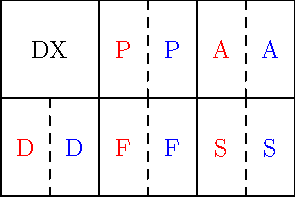
\includegraphics[scale=1.2]{grid.pdf}
      \caption{\label{f_grid}地图网格信息示意图}
\end{figure}
其中, DX 为地形的名称, 红色表示我方 (\lcode{opt = 0}), 蓝色表示敌方 (\lcode{opt = 1}).
显示 P 表示有人位于此位置, 否则不显示. A 表示该位置存在攻击辅助效果.
D 表示该位置存在防御辅助效果. F 表示该位置存在飞行辅助效果, 即移动量消耗值被修改.
S 表示该位置存在远程攻击无效的辅助效果. 使用上下左右箭头键或类似 vim 中的 h(左), j(下), k(上), l(右) 键
可以在地图上移动光标. 当地图大小超过可显示范围时, 可使用 w, b, d, u 分别向右, 左, 下, 上滚动半个屏幕. 
使用 Ctrl-d, Ctrl-u 可达到使用 d, u 相同的效果. 屏幕右端的 XScroll, YScroll 部分
显示了当前窗口在整个地图中的位置. 使用 Tab 键可以自动使光标移动到下一个本回合当前操作方还尚未行动的人物所在的位置.

屏幕右侧会跟随光标的移动显示位置和人员信息. 最上一个窗口显示
地形名称, 移动量消耗, 人物名称, 操作方 (OptA, OptB), 生命值, 本回合是否已行动完毕, 攻击力, 防御力, 移动速度 (每回合移动值).
第二个窗口显示一个表格, 表示该位置的辅助效果. OptA, OptB 分别表示对两方的不同辅助效果. Value 表示效果值, Dur. 表示效果的剩余持续时间.
第三个窗口显示坐落于该位置的人物所掌握的全部技术名称. 最下面一个窗口为操作提示. 

当操作提示选择一个人物或位置时, 首先移动光标到特定位置, 然后通过 Enter 键确定选择该位置或人物. 
当选择移动目的地或技术的目标位置时, 允许选择的区域会做特殊显示. 在选择移动目的地时, 
按下 q 键可取消选择而退回上一步. 当出现 Select tech 的提示时, 输入数字键可选择待执行的技术, 
此时若键入 q, 则对该人物只做移动而不执行任何技术. 在选择人物进行操作的状态下, 
按下 t 可提前终止本方的本回合操作. 按下 q 可退出游戏. 
当操作提示出现 `?' 时, 按 y 表示确认, n 表示取消. 当对某个人物造成伤害时, 对应网格 P 字的位置会临时显示伤害值.

\section{UI 接口定义}
\label{s_ui}
UI 接口包括两个, 分别如下定义.
\begin{lstlisting}
type UINote interface {
	/* DoTech triger before HPDown, Loc.. */
	DoTech (itech, p_src, p_obj, l_obj int)
	HPDown (ip, loc, hp, dhp int)
	PeopleIn (ip, loc int)
	PeopleOut (ip, loc int)
	/* PeopleMove trigger after PeopleStep */
	PeopleMove (ip, loc_start, loc_end int)
	PeopleStep (ip, loc, dir int)
	/* att_def: 0: att; 1: def */
	LocBuf (loc, att_def, val, dur int)
	LocFly (loc, weight, dur int)
	LocDisableLong (loc, dur int)

	LoadMapDone ()
	GameStart ()
	/* win_opt == -1: 退出*/ 
	GameOver (win_opt int) 
}

type UISelect interface {
	TurnStart (opt int)
      /* return -1 to quit, -2 to end turn (only for SOS_PEOPLE) 
	* valid_loc is only valid in SOS_MOVE_OBJ status
	* */
	SelObj (status SelObjStatus, itech int, valid_loc []int) int 
      /* return -1 to give up tech use */
	SelTech (ip int) int
	/* return true to confirm quit */
	Confirm (msg string) bool 
}
\end{lstlisting}
其中, \lcode{UINote} 收集了所有通知操作, \lcode{UISelect} 收集了所有需要用户交互的操作. 
需要定义两个 \lcode{UISelect} 接口的实现以支持两个操作方. 以下分别说明各接口函数.

\lcode{Init} 函数完成后会调用 \lcode{LoadMapDone} 函数. \lcode{Do} 函数会首先调用 \lcode{GameStart} 函数.
\lcode{Do} 函数返回前会调用 \lcode{GameOver} 函数. 其中 \lcode{win_opt} 为 $-1$ 表示中途退出. 
取 $0, 1$ 则表示相应操作方取胜.
当每个操作方的回合开始时, 会调用 \lcode{TurnStart} 函数. 其中 \lcode{opt} 为操作方编号.

\begin{lstlisting}
DoTech (itech, p_src, p_obj, l_obj int)
\end{lstlisting}
用于通知技术被施用. \lcode{itech} 为技术编号. \lcode{p_src} 为施用人, \lcode{l_obj} 为目标对象位置, \lcode{p_obj} 
为目标对象人物, 可为 $-1$.

\begin{lstlisting}
HPDown (ip, loc, hp, dhp int)
\end{lstlisting}
用于通知某人受到伤害. \lcode{ip} 为受害人, \lcode{loc} 为受害人所在位置, 
\lcode{hp} 为受害人伤害前的生命值,  \lcode{dhp} 为伤害值.

\begin{lstlisting}
PeopleIn (ip, loc int)
\end{lstlisting}
用于通知某人加入战场, 在 \lcode{Init} 函数中被调用.
\lcode{ip} 表示加入人, \lcode{loc} 表示加入位置.

\begin{lstlisting}
PeopleOut (ip, loc int)
\end{lstlisting}
用于通知某人生命值归零后撤离战场, \lcode{ip} 表示待撤离的人, 
\lcode{loc} 表示从哪个位置撤离.

\begin{lstlisting}
/* PeopleMove trigger after PeopleStep */
PeopleMove (ip, loc_start, loc_end int)
\end{lstlisting}
用于通知某人 \lcode{ip} 从位置 \lcode{loc_start} 移动到位置 \lcode{loc_end}. 该函数会在调用 \lcode{PeopleStep} 之后被调用.

\begin{lstlisting}
PeopleStep (ip, loc, dir int)
\end{lstlisting}
用于通知某人 \lcode{ip} 从位置 \lcode{loc} 出发移动一步. \lcode{dir} 用于指示移动的方向. 移动方向的定义可参见图 \ref{f_dir}.
\begin{figure}
      \centering
      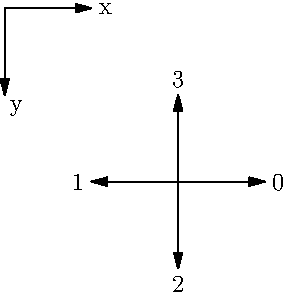
\includegraphics[scale=1]{dir.pdf}
      \caption{\label{f_dir}方向编号的含义}
\end{figure}

人物每一次移动会先分解为若干步 \lcode{PeopleStep} 发送给 UI, 然后再针对本次整体的移动行为发送一个 \lcode{PeopleMove} 消息给 UI.
最后在实际修改人物和地图的相关属性.

\begin{lstlisting}
/* att_def: 0: att; 1: def */
LocBuf (loc, att_def, val, dur int)
\end{lstlisting}
用于通知某个位置 \lcode{loc} 获得了攻防的辅助效果. \lcode{att_def} 用于指明攻或防, 
\lcode{val} 为实际获得的辅助值, \lcode{dur} 为辅助效果的持续时间.

\begin{lstlisting}
LocFly (loc, weight, dur int)
\end{lstlisting}
用于通知某个位置 \lcode{loc} 获得了飞行辅助效果. 该位置的移动量消耗将被修改为 \lcode{weight}, 持续时间为 \lcode{dur}.

\begin{lstlisting}
LocDisableLong (loc, dur int)
\end{lstlisting}
用于通知某个位置 \lcode{loc} 获得了远程攻击无效的辅助效果, 持续时间 \lcode{dur}.

上述所有通知消息均发生在实际修改人员或地图的属性之前. 或者说 UI
在收到通知消息时, 人员或地图的属性还保留旧的值.

\begin{lstlisting}
/* return -1 to quit, -2 to end turn (only for SOS_PEOPLE) 
* valid_loc is only valid in SOS_MOVE_OBJ status
* */
SelObj (status SelObjStatus, itech int, valid_loc []int) int 
\end{lstlisting}
用于从用户获取一个地图上的选择位置. \lcode{status} 为需要做出选择时的当前状态, 可取自常数  
\begin{lstlisting}
type SelObjStatus int
const (
	SOS_PEOPLE SelObjStatus = 0
	SOS_MOVE_OBJ SelObjStatus = 1
	SOS_TECH_OBJ SelObjStatus = 2
)
\end{lstlisting}
其中, \lcode{SOS_PEOPLE} 表示选择一个人物进行移动, 对应第 \ref{s_intro} 节所述的第 \ref{step_sel} 步.
\lcode{SOS_MOVE_OBJ} 表示选择人物的移动目的地, 对应第 \ref{s_intro} 节所述的第 \ref{step_move} 步. 
\lcode{SOS_TECH_OBJ} 表示选择技能的目标位置, 对应第 \ref{s_intro} 节所述的第 \ref{step_obj} 步. 
\lcode{itech} 仅在 \lcode{SOS_TECH_OBJ} 时有效, 指明所使用的技能编号.
\lcode{valid_loc} 仅在 \lcode{SOS_MOVE_OBJ} 时有效, 包含所有允许的移动位置.
函数需要返回用户所选择的位置编号. 如果返回 $-1$, 
在状态 \lcode{SOS_PEOPLE} 表示中途退出游戏;
在状态 \lcode{SOS_MOVE_OBJ} 表示取消操作该人物, 返回选择操作人物界面;
在状态 \lcode{SOS_TECH_OBJ} 表示取消使用该技能, 返回选择技能界面.
在状态 \lcode{SOS_PEOPLE}, 如果返回 $-2$, 则表示提前终止本方的本回合. (剩余可行动人物都取消行动)

\begin{lstlisting}
/* return -1 to give up tech use */
SelTech (ip int) int
\end{lstlisting}
用于从用户获取为某个人物 \lcode{ip} 选择一项待执行的技术. 
返回所选技术在 \lcode{people[ip].tech} 数组中的顺序编号 (注意不是全局技术编号).
返回 $-1$ 表示不使用任何技术 (仅移动).

\begin{lstlisting}
/* return true to confirm */
Confirm (msg string) bool 
\end{lstlisting}
用于向用户发送一条信息并询问用户是否的答复. 中途退出游戏或结束本回合时会调用该函数.

\end{document}

